\documentclass[conference]{IEEEtran}
\IEEEoverridecommandlockouts

\usepackage[utf8]{inputenc}
\usepackage[T1]{fontenc}
\usepackage{amsmath, amsfonts, amssymb}
\usepackage{graphicx}
\usepackage{booktabs}
\usepackage{hyperref}
\usepackage{caption}
\usepackage{subcaption}
\usepackage{float}
\usepackage{listings}
\usepackage{xcolor}
\usepackage{bm}

\definecolor{codegreen}{rgb}{0,0.6,0}
\definecolor{codegray}{rgb}{0.5,0.5,0.5}
\definecolor{codepurple}{rgb}{0.58,0,0.82}
\definecolor{backcolour}{rgb}{0.95,0.95,0.92}

\lstdefinestyle{mystyle}{
    backgroundcolor=\color{backcolour},
    commentstyle=\color{codegreen},
    keywordstyle=\color{magenta},
    numberstyle=\tiny\color{codegray},
    stringstyle=\color{codepurple},
    basicstyle=\ttfamily\footnotesize,
    breakatwhitespace=false,
    breaklines=true,
    captionpos=b,
    keepspaces=true,
    numbers=left,
    numbersep=5pt,
    showspaces=false,
    showstringspaces=false,
    showtabs=false,
    tabsize=2
}
\lstset{style=mystyle}

\begin{document}

\title{Hybrid Zero Dynamics-Based Gait Design and Feedback Linearization Control of a 3-Link Planar Bipedal Robot}

\author{
\IEEEauthorblockN{Shriman Raghav Srinivasan, Gautham Ramkumar, Prasath Saravanan, and Garett Christopher}
\IEEEauthorblockA{\textit{Department of Electrical and Computer Engineering}\\
\textit{Northeastern University}\\
Boston, Massachusetts \\
\{srinivasan.shrim, ramkumar.g, saravanan.pras, christopher.g\}@northeastern.edu}
}

\maketitle

\begin{abstract}
This report details the complete modeling, gait design, and control of a 3-link planar bipedal robot using the Hybrid Zero Dynamics (HZD) framework. Starting from first principles, we derive the full continuous swing-phase dynamics via the Lagrangian formalism, construct the inertia, Coriolis, and gravity matrices explicitly, and define an impact map using conservation of angular momentum to handle the instantaneous leg-swap event. Virtual constraints are then imposed on the two actuated joints by parameterizing their desired trajectories as 4th-order B\'ezier polynomials of a monotonically increasing gait timing variable. The system is projected onto a 2-DOF zero dynamics manifold, whose periodic orbit is optimized for minimum quadratic control effort using MATLAB's \texttt{fmincon}. An exact output feedback linearization controller, computing the full Lie derivative hierarchy and the decoupling matrix online, drives the full 6-state system onto this manifold. Full dynamic simulation over 15 steps confirms asymptotic convergence to a stable limit cycle, a walking speed of $\sim\!1.73$ m/s, and a Mechanical Cost of Transport (MCOT) of 1.1584.
\end{abstract}

\begin{IEEEkeywords}
Bipedal locomotion, Hybrid Zero Dynamics, Feedback linearization, B\'ezier polynomial, Trajectory optimization, Underactuated robotics, Limit cycle, Poincar\'e map.
\end{IEEEkeywords}

% =========================================================
\section{Introduction}
% =========================================================

Achieving stable, energy-efficient locomotion in legged robots is a fundamental challenge that demands a principled treatment of hybrid dynamics, underactuation, and high-dimensional state spaces. Bipedal walkers are especially demanding: each step involves a continuous swing phase governed by Lagrangian mechanics, followed by an instantaneous, energy-dissipative foot-strike event. The resulting \emph{hybrid dynamical system} cannot be stabilized by classical linear methods and instead requires a control architecture that explicitly accounts for this discontinuous, underactuated structure.

Classical approaches to bipedal stability, most notably the \emph{Zero Moment Point} (ZMP) criterion~\cite{hirai1998}, enforce balance by constraining the net ground-reaction moment to lie within the support polygon at every instant. This quasi-static strategy guarantees fall prevention but does so at a significant energetic and kinematic cost: the natural pendulum-like swing of the legs must be continuously suppressed, producing characteristically slow and stiff gaits with high mechanical cost of transport.

The \emph{Hybrid Zero Dynamics} (HZD) framework~\cite{westervelt,grizzle} is founded on a geometrically principled alternative. Rather than opposing the passive dynamics, HZD exploits them by confining the closed-loop system to an invariant, low-dimensional submanifold of the state space, the \emph{zero dynamics manifold} $\mathcal{Z}$. On $\mathcal{Z}$, the full 6-state hybrid system reduces to a scalar hybrid oscillator driven entirely by the unactuated stance-leg coordinate. The central insight is that designing a stable limit cycle for this reduced 2-state system, and then proving that the manifold is rendered invariant and attractive by feedback, is sufficient to guarantee exponential orbital stability of the full-order walking gait~\cite{westervelt}. This separation of concerns---gait design on the manifold and stabilization of the manifold by control---is what makes HZD both analytically tractable and practically effective.

Experimentally, HZD has produced some of the most efficient and dynamic gaits achieved on physical hardware: planar 5-link walkers~\cite{grizzle,plestan2003}, the 3D biped ATRIAS operating at human walking speeds~\cite{ramezani2013}, and human-inspired controllers for prosthetic legs~\cite{ames}. The framework's scalability from 2D to 3D and from walking to running makes it the dominant theoretical paradigm for underactuated bipedal control.

This report presents the full HZD design and implementation pipeline for a 3-link planar biped. We derive the continuous and impact dynamics from first principles (Section~\ref{sec:model}), construct time-invariant virtual constraints via 4th-order B\'ezier polynomials and derive the scalar zero dynamics (Section~\ref{sec:gait}), formulate and solve the constrained periodic-gait optimization problem (Section~\ref{sec:opt}), implement exact input-output feedback linearization with online Lie derivative computation (Section~\ref{sec:control}), and validate the design through a 15-step full-state simulation with Poincar\'e stability analysis and MCOT efficiency evaluation (Sections~\ref{sec:sim}--\ref{sec:efficiency}).

% =========================================================
\section{Robot Model} \label{sec:model}
% =========================================================

\subsection{Physical Description and Parameters}

The robot is modeled as a 3-link planar biped operating in the sagittal plane. It consists of two legs of equal length $r$, each carrying a point mass $m$ at its midpoint, connected at a hip joint of mass $M_h$. A torso of length $l$ and mass $M_t$ is rigidly attached to the hip. The feet are modeled as point contacts with no ankle actuation. It is assumed that at most one foot contacts the ground at any time, that ground contact is rigid and frictionless (no slipping), and that the leg-swap at foot-strike is instantaneous.

\begin{table}[htbp]
    \centering
    \caption{Physical parameters of the 3-link bipedal robot.}
    \label{tab:params}
    \begin{tabular}{llc}
        \toprule
        \textbf{Parameter} & \textbf{Symbol} & \textbf{Value} \\
        \midrule
        Leg link length      & $r$       & 1 m \\
        Point mass (each leg)& $m$       & 5 kg \\
        Hip mass             & $M_h$     & 15 kg \\
        Torso mass           & $M_t$     & 10 kg \\
        Torso length         & $l$       & 0.5 m \\
        Gravity              & $g$       & 9.81 m/s$^2$ \\
        Total mass           & $M_{tot}$ & 35 kg \\
        \bottomrule
    \end{tabular}
\end{table}

\subsection{Generalized Coordinates}

The configuration space is $\mathcal{Q} = \mathbb{R}^3$ with generalized coordinates:
\begin{equation}
    q = \begin{bmatrix} q_1 \\ q_2 \\ q_3 \end{bmatrix}
\end{equation}
where $q_1$ is the absolute angle of the stance leg measured from the negative $y$-axis (downward vertical), $q_2$ is the inter-leg angle (swing leg relative to the stance leg), and $q_3$ is the torso angle relative to the stance leg. The origin is fixed at the stance foot contact point. The sign convention gives $q_1 < 0$ when the stance leg leans forward, which is the typical walking configuration.

The absolute angles of the three links are:
\begin{align}
    \theta_1^{abs} &= q_1 \label{eq:abs1}\\
    \theta_2^{abs} &= q_1 + q_2 \label{eq:abs2}\\
    \theta_3^{abs} &= q_1 + q_3 - \pi \label{eq:abs3}
\end{align}
The torso offset of $\pi$ in~\eqref{eq:abs3} reflects that the torso points upward from the hip while the legs point downward.

\subsection{Forward Kinematics}

The Cartesian positions of each mass in the inertial frame, with the origin at the stance foot, are:
\begin{align}
    p_{M_h} &= r \begin{bmatrix} \sin(-q_1) \\ \cos(-q_1) \end{bmatrix} \label{eq:pmh}\\
    p_{M_t} &= p_{M_h} + l \begin{bmatrix} \sin(-q_1+\pi-q_3) \\ \cos(-q_1+\pi-q_3) \end{bmatrix} \label{eq:pmt}\\
    p_{m_1} &= \frac{r}{2} \begin{bmatrix} \sin(-q_1) \\ \cos(-q_1) \end{bmatrix} \label{eq:pm1}\\
    p_{m_2} &= p_{M_h} + \frac{r}{2} \begin{bmatrix} \sin(q_1+q_2) \\ -\cos(q_1+q_2) \end{bmatrix} \label{eq:pm2}\\
    P_2     &= p_{M_h} + r \begin{bmatrix} \sin(q_1+q_2) \\ -\cos(q_1+q_2) \end{bmatrix} \label{eq:P2}
\end{align}
where $P_2$ is the swing foot tip position. Impact occurs when the vertical component $[P_2]_y = 0$.

The velocity of each mass is obtained via the velocity Jacobians:
\begin{equation}
    \dot{p}_i = J_{v_i}(q)\,\dot{q}, \qquad J_{v_i} = \frac{\partial p_i}{\partial q} \in \mathbb{R}^{2\times 3}
\end{equation}
These Jacobians are computed symbolically and used to assemble the inertia matrix.

The system center of mass is:
\begin{equation}
    p_{cm} = \frac{m\,p_{m_1} + m\,p_{m_2} + M_h\,p_{M_h} + M_t\,p_{M_t}}{M_{tot}}
\end{equation}

\subsection{Equations of Motion via Lagrangian Mechanics}

The Lagrangian is $\mathcal{L}(q,\dot{q}) = K(q,\dot{q}) - V(q)$.

\subsubsection{Kinetic Energy}
\begin{equation}
    K = \frac{1}{2}\dot{q}^T D(q)\,\dot{q}
\end{equation}
The symmetric positive-definite inertia matrix $D(q) \in \mathbb{R}^{3\times 3}$ is:
\begin{equation}
    D(q) = \sum_{i \in \mathcal{M}} m_i\, J_{v_i}^T(q)\, J_{v_i}(q) \label{eq:inertia}
\end{equation}
where $\mathcal{M} = \{m_1, m_2, M_h, M_t\}$ with masses from Table~\ref{tab:params}.

\subsubsection{Potential Energy}
\begin{equation}
    V(q) = g\sum_{i \in \mathcal{M}} m_i\, [p_i]_y
\end{equation}
where $[p_i]_y$ is the vertical component of the $i$-th mass position.

\subsubsection{Equations of Motion}
Applying $\frac{d}{dt}\frac{\partial\mathcal{L}}{\partial\dot{q}} - \frac{\partial\mathcal{L}}{\partial q} = \Gamma$ yields the standard manipulator form:
\begin{equation}
    D(q)\ddot{q} + C(q,\dot{q})\dot{q} + G(q) = B\,u \label{eq:eom}
\end{equation}
The Coriolis/centrifugal matrix entries are computed via Christoffel symbols:
\begin{equation}
    C_{kj}(q,\dot{q}) = \sum_{i=1}^{3} \frac{1}{2}\!\left(\frac{\partial D_{kj}}{\partial q_i} + \frac{\partial D_{ki}}{\partial q_j} - \frac{\partial D_{ij}}{\partial q_k}\right)\!\dot{q}_i
\end{equation}
The gravity vector is $G(q) = \partial V/\partial q$, and the input matrix
\begin{equation}
    B = \begin{bmatrix} 0 & 0 \\ 1 & 0 \\ 0 & 1 \end{bmatrix} \label{eq:B}
\end{equation}
maps control torques $u = [u_2,\, u_3]^T$ at the two hip joints to generalized forces. The stance ankle ($q_1$) is unactuated, making this a 1-degree-of-underactuation system.

\subsubsection{Control-Affine State-Space Form}
With state $x = [q^T,\, \dot{q}^T]^T \in \mathbb{R}^6$, the swing-phase dynamics take the control-affine form:
\begin{equation}
    \dot{x} = f(x) + g(x)\,u \label{eq:affine}
\end{equation}
where:
\begin{align}
    f(x) &= \begin{bmatrix} \dot{q} \\ D^{-1}(q)\bigl(-C(q,\dot{q})\dot{q} - G(q)\bigr) \end{bmatrix} \\
    g(x) &= \begin{bmatrix} 0_{3\times 2} \\ D^{-1}(q)\,B \end{bmatrix}
\end{align}

\subsection{Impact Model and Hybrid System}

Walking is a \emph{hybrid} dynamical system. The complete model is:
\begin{equation}
    \Sigma:\; \begin{cases} \dot{x} = f(x) + g(x)u, & x^- \notin \mathcal{S} \\ x^+ = \Delta(x^-), & x^- \in \mathcal{S} \end{cases}
\end{equation}

\subsubsection{Impact Guard Surface}
\begin{equation}
    \mathcal{S} = \bigl\{(q,\dot{q})\in T\mathcal{Q} \;\big|\; [P_2]_y(q) = 0,\; [P_2]_x(q) > 0\bigr\}
\end{equation}

\subsubsection{Impact Map $\Delta$}

Foot-strike is modeled as a rigid, instantaneous, perfectly plastic collision with no rebound or slip. At the moment of impact, the swing foot becomes the new stance point and the legs exchange roles. Two steps are required: a velocity reset via angular momentum conservation, and a coordinate relabeling that maps pre-impact single-support coordinates to post-impact ones.

\textbf{Step 1 — Velocity reset.}
To correctly account for impulsive forces acting at the new contact point, the pinned single-support model is embedded into a floating-base \emph{extended} model. Define the floating-base center-of-mass map $p_e = \Upsilon_e(q_s) \in \mathbb{R}^2$ and the extended coordinate vector $q_e = [q_s^T, p_e^T]^T \in \mathbb{R}^5$. The extended pre-impact velocity satisfies:
\begin{equation}
    \dot{q}_e^- = \begin{bmatrix} I_{3\times3} \\ \frac{\partial \Upsilon_e}{\partial q_s}(q_s^-) \end{bmatrix}\dot{q}_s^- \triangleq \Gamma_e(q_s^-)\,\dot{q}_s^-
\end{equation}
At impact, the new stance foot is instantaneously pinned, and the impulsive ground-reaction force $F_2$ acts at the swing foot tip $P_2(q_e)$. The impulse-momentum law for the extended system yields:
\begin{equation}
    D_e(q_e^-)\,(\dot{q}_e^+ - \dot{q}_e^-) = E_2^T(q_e^-)\,F_2
\end{equation}
where $D_e \in \mathbb{R}^{5\times5}$ is the extended inertia matrix and $E_2 = \partial P_2/\partial q_e$ maps extended velocities to swing-tip velocity. Imposing the no-penetration condition $E_2\,\dot{q}_e^+ = 0$ and eliminating $F_2$:
\begin{equation}
    \dot{q}_s^+ = \bigl[I - D_e^{-1}E_2^T(E_2 D_e^{-1}E_2^T)^{-1}E_2\bigr]\,\Gamma_e\,\dot{q}_s^- \label{eq:impact_vel}
\end{equation}

\textbf{Step 2 — Coordinate relabeling.}
After impact, what was the swing leg becomes the new stance leg. This is effected by the permutation (switching) matrix $R$:
\begin{equation}
    q^+ = R\,q^-
\end{equation}
where $R$ swaps the leg indices $(q_2 \leftrightarrow -q_2)$ and reflects the stance angle $(q_1 \to -q_1 - q_2)$ to maintain the coordinate convention with the new ground contact as origin.

The combined impact map $\Delta: (q^-, \dot{q}^-) \mapsto (q^+, \dot{q}^+)$ is strictly energy-dissipative, satisfying $K(q^+, \dot{q}^+) < K(q^-, \dot{q}^-)$ for all non-degenerate collisions. A sustainable periodic gait must supply, averaged over each step, precisely this dissipated kinetic energy through the actuated joints.

% =========================================================
\section{Gait Design via Hybrid Zero Dynamics} \label{sec:gait}
% =========================================================

\subsection{Virtual Constraints and Output Functions}

The fundamental idea of HZD gait design is to reduce the $2n$-dimensional hybrid state space to a 2-dimensional invariant submanifold by imposing $n-1$ \emph{virtual constraints}: smooth, holonomic output functions $y = h(q) \in \mathbb{R}^{n-1}$ that are driven to zero by feedback. The term \emph{virtual} distinguishes these from physical (mechanical) constraints: they arise purely from closed-loop control action and can therefore be designed for optimal gait properties rather than being fixed by hardware geometry~\cite{westervelt}.

For the 3-link biped with $n=3$ degrees of freedom and 2 actuated joints, we impose $n-1 = 2$ virtual constraints. Define the output vector as:
\begin{equation}
    y = h(q) = H_0 q - h_d(\sigma(q)) = \begin{bmatrix} q_2 - b_2(\sigma(q)) \\ q_3 - b_3(\sigma(q)) \end{bmatrix} \label{eq:output}
\end{equation}
where $H_0 = \begin{bmatrix}0&1&0\\0&0&1\end{bmatrix}$ selects the actuated coordinates, $b_2(\sigma)$ and $b_3(\sigma)$ are desired joint trajectories parameterized by the scalar gait timing variable $\sigma \in [0,1]$, and $h_d = [b_2(\sigma), b_3(\sigma)]^T$ is the B\'ezier-parameterized reference trajectory. The constraint $y = 0$ makes $q_2$ and $q_3$ \emph{slaves} to $q_1$ through the common phasing variable $\sigma(q_1)$, effectively reducing the actuated DOFs to zero and leaving only the unactuated $q_1$ to evolve freely under gravity.

\subsection{Gait Timing Variable}

The timing variable must be monotonically increasing through the swing phase and reset at each impact, without requiring a clock. Using the unactuated coordinate $q_1$:
\begin{equation}
    \sigma(q) = \frac{q_1 - q_1^+}{q_1^- - q_1^+} = \frac{q_1 - q_1^+}{\Delta q} \label{eq:s}
\end{equation}
where $q_1^+$ is the post-impact stance angle, $q_1^-$ is the pre-impact stance angle, and $\Delta q = q_1^- - q_1^+ < 0$. Since $q_1$ sweeps monotonically under the gravity-driven inverted pendulum dynamics, $\sigma$ runs smoothly from 0 to 1 across each step.

\subsection{B\'ezier Polynomial Trajectories}

The desired joint trajectories are parameterized as 4th-order ($M=4$) B\'ezier polynomials:
\begin{equation}
    b_i(\sigma) = \sum_{k=0}^{4} \alpha_k^{(i)} \binom{4}{k} \sigma^k (1-\sigma)^{4-k} \label{eq:bezier}
\end{equation}
where $\alpha_k^{(i)}$ are the B\'ezier control points for output $i \in \{2,3\}$.

\subsubsection{Boundary Condition Pinning}
B\'ezier polynomials satisfy $b(0)=\alpha_0$, $b(1)=\alpha_4$, and endpoint derivative relations $b'(0)=M(\alpha_1-\alpha_0)$, $b'(1)=M(\alpha_4-\alpha_3)$. By defining a symmetric gait and utilizing the impact coordinate map, the endpoints of the trajectory are determined. The optimization effectively tunes the interior control points. For this design, the full parameter optimization vector spans 8 dimensions: the pre-impact zero-dynamics states $(q_1^-, \dot{q}_1^-)$ and the 3rd to 5th coefficients of the two B\'ezier curves, representing $\alpha_2$, $\alpha_3$, and $\alpha_4$ in zero-indexed form.

The full optimization vector is:
\begin{equation}
\begin{split}
    \bm{f} = \bigl[& q_1^-,\;\dot{q}_1^-,\;\alpha_2^{(2)},\;\alpha_3^{(2)},\;\alpha_4^{(2)}, \\
                   & \alpha_2^{(3)},\;\alpha_3^{(3)},\;\alpha_4^{(3)}\bigr]^T \in \mathbb{R}^8
\end{split}
\label{eq:fvec}
\end{equation}
The remaining starting coefficients are mapped due to symmetric walking principles: $\alpha_0^{(2)} = -\alpha_4^{(2)}$, $\alpha_1^{(2)} = -\alpha_3^{(2)}$, $\alpha_0^{(3)} = \alpha_4^{(3)} - \alpha_4^{(2)}$, and $\alpha_1^{(3)} = -\alpha_3^{(3)} + 2\alpha_2^{(3)}$.

\subsubsection{B\'ezier Derivatives}
The derivative of $b_i$ with respect to $\sigma$ is needed for the Lie derivative computation:
\begin{equation}
    \frac{\partial b_i}{\partial \sigma} = M \sum_{k=0}^{M-1} (\alpha_{k+1}^{(i)} - \alpha_k^{(i)}) \binom{M-1}{k} \sigma^k (1-\sigma)^{M-1-k}
\end{equation}
The second derivative $\partial^2 b_i/\partial \sigma^2$ enters the curvature term of the zero dynamics.

\subsection{Zero Dynamics Manifold and Coordinate Transformation}

\subsubsection{Diffeomorphism to Normal Form}
To formally derive the zero dynamics, we apply the diffeomorphism $\Phi: T\mathcal{Q} \to \mathbb{R}^6$ defined by:
\begin{equation}
    \Phi(q,\dot{q}) = \begin{bmatrix} \eta_1 \\ \eta_2 \\ \xi_1 \\ \xi_2 \end{bmatrix}
    = \begin{bmatrix} h(q) \\ L_f h(x) \\ \sigma(q) \\ \dot{\sigma}(q,\dot{q}) \end{bmatrix}
    \label{eq:diffeo}
\end{equation}
where $(\eta_1, \eta_2) \in \mathbb{R}^4$ are the constraint coordinates (tracking errors and their rates) and $(\xi_1, \xi_2) \in \mathbb{R}^2$ are the internal coordinates on the manifold. Since the system has uniform vector relative degree $\{2,2\}$, this mapping is a local diffeomorphism wherever $\det(L_g L_f h) \neq 0$~\cite{westervelt}. In the new coordinates, the dynamics decompose as:
\begin{align}
    \dot{\eta}_1 &= \eta_2 \\
    \dot{\eta}_2 &= L_f^2 h + (L_g L_f h)\,u \\
    \dot{\xi}_1  &= \xi_2 \label{eq:xi1dot}\\
    \dot{\xi}_2  &= L_f^2 \sigma + (L_g L_f \sigma)\,u^* \label{eq:xi2dot}
\end{align}
Setting $u$ to enforce $\eta_1 \to 0, \eta_2 \to 0$ renders the $\eta$-subsystem stable. When $\eta = 0$ exactly, $(L_g L_f \sigma)\,u^*$ evaluates to the feedforward torque that maintains the manifold, and~\eqref{eq:xi1dot}--\eqref{eq:xi2dot} become the \emph{zero dynamics}: a 2-state autonomous system in $(\xi_1, \xi_2) = (\sigma, \dot{\sigma})$.

\subsubsection{Scalar Zero Dynamics ODE}
The zero dynamics manifold is:
\begin{equation}
    \mathcal{Z} = \bigl\{x \in \mathbb{R}^6 \;\big|\; h(q) = 0,\; L_f h(x) = 0\bigr\}
\end{equation}
On $\mathcal{Z}$: $q_i = b_i(\sigma(q_1))$ for $i \in \{2,3\}$, so the time derivatives are:
\begin{equation}
    \dot{q}_i = \frac{1}{\Delta q}\frac{\partial b_i}{\partial \sigma}\,\dot{q}_1 \triangleq \beta_i^{(1)}(q_1)\,\dot{q}_1
\end{equation}
\begin{equation}
    \ddot{q}_i = \beta_i^{(1)}\ddot{q}_1 + \frac{1}{(\Delta q)^2}\frac{\partial^2 b_i}{\partial \sigma^2}\dot{q}_1^2 \triangleq \beta_i^{(1)}\ddot{q}_1 + \beta_i^{(2)}\dot{q}_1^2
\end{equation}
Substituting these expressions into the first (unactuated) row of~\eqref{eq:eom} and solving for $\ddot{q}_1$ yields the scalar zero dynamics ODE:
\begin{equation}
    \ddot{q}_1 = \frac{-[C\dot{q}+G]_1 - D_{12}\beta_2^{(2)}\dot{q}_1^2 - D_{13}\beta_3^{(2)}\dot{q}_1^2}
                      {D_{11} + D_{12}\beta_2^{(1)} + D_{13}\beta_3^{(1)}} \label{eq:zdyn}
\end{equation}
where $[\cdot]_1$ denotes the first element (unactuated row), $D_{ij} \equiv [D(q)]_{ij}$, and all quantities are evaluated on $\mathcal{Z}$ (i.e., $q_2 = b_2(\sigma)$, $q_3 = b_3(\sigma)$). Note that the actuator inputs $u$ do not appear: \eqref{eq:zdyn} is a \emph{free} nonlinear oscillator. A stable periodic orbit of~\eqref{eq:zdyn} that maps to itself under the reduced impact map $\Delta_{ZD}: (\xi_1^-, \xi_2^-) \mapsto (\xi_1^+, \xi_2^+)$ constitutes a valid, self-consistent walking gait.

% =========================================================
\section{Gait Optimization} \label{sec:opt}
% =========================================================

\subsection{Optimization Problem Formulation}

The gait design problem is a constrained nonlinear program over the 8-parameter vector $\bm{f}$ defined in~\eqref{eq:fvec}. The remaining B\'ezier control points ($\alpha_0, \alpha_1$) are determined by the boundary mapping conditions.

\textbf{Objective:} minimize average quadratic control effort per step:
\begin{equation}
    J(\bm{f}) = \frac{1}{t_f - t_0} \int_{t_0}^{t_f} \|u^*(\tau)\|^2\, d\tau \label{eq:cost}
\end{equation}
where $u^*$ is the torque required to maintain the zero dynamics (i.e., to keep $y \equiv 0$ along the trajectory), and the integral spans one step of the zero dynamics simulation.

\textbf{Constraints}:
\begin{enumerate}
    \item \emph{Hybrid periodicity (equality).} For a fixed point of the Poincar\'e map $\mathcal{P}$, the zero dynamics state must be self-consistent after one complete step and the associated impact:
    \begin{equation}
        \mathcal{P}\!\begin{pmatrix} q_1^- \\ \dot{q}_1^- \end{pmatrix}
        \triangleq \Delta_{ZD}\!\left(\phi_{ZD}^{T}\!\begin{pmatrix} q_1^+ \\ \dot{q}_1^+ \end{pmatrix}\right)
        \stackrel{!}{=}
        \begin{pmatrix} q_1^- \\ \dot{q}_1^- \end{pmatrix}
    \end{equation}
    where $\phi_{ZD}^T$ is the flow map of~\eqref{eq:zdyn} from $\sigma=0$ to $\sigma=1$. This imposes two scalar nonlinear equality constraints.

    \item \emph{Swing-foot ground clearance (inequality).} The vertical component of the swing-foot tip must remain non-negative throughout the entire step:
    \begin{equation}
        [P_2]_y\!\bigl(q(\sigma)\bigr) \geq 0, \quad \forall\, \sigma \in [0,1]
    \end{equation}
    This prevents the swing foot from clipping the ground during mid-flight, and is enforced by evaluating $[P_2]_y$ within \texttt{fmincon}'s nonlinear constraint function.

    \item \emph{Kinematic bounds (box constraints).} The parameters are bounded appropriately to prevent degenerate solutions.
\end{enumerate}

The constrained nonlinear program is solved with MATLAB's \texttt{fmincon} using the interior-point algorithm.

\subsection{Optimized Results}

The optimizer converged to a highly efficient periodic orbit. The optimal parameter vector is:
\begin{equation}
\begin{split}
    \bm{f}^* = \bigl[& -0.4907,\; -2.3947,\; 0.3053,\; 0.6256, \\
                     & 0.8814,\; 2.6360,\; 2.7919,\; 2.9537 \bigr]^T
\end{split}
\end{equation}
corresponding to $q_1^* = -0.4907$ rad, $\dot{q}_1^* = -2.3947$ rad/s. The coefficients for the B\'ezier curves map to a fast-paced and natural walking trajectory.

\begin{table}[htbp]
    \centering
    \caption{All B\'ezier control points at the optimal solution.}
    \label{tab:bezier}
    \begin{tabular}{lccccc}
        \toprule
        \textbf{Output} & $\alpha_0$ & $\alpha_1$ & $\alpha_2$ & $\alpha_3$ & $\alpha_4$ \\
        \midrule
        $b_2(\sigma)$ & -0.8814 & -0.6256 & 0.3053 & 0.6256 & 0.8814 \\
        $b_3(\sigma)$ & 2.0723 & 2.4801 & 2.6360 & 2.7919 & 2.9537 \\
        \bottomrule
    \end{tabular}
\end{table}

% =========================================================
\section{Feedback Linearization Controller} \label{sec:control}
% =========================================================

\subsection{Control Objective}

The diffeomorphism~\eqref{eq:diffeo} reveals that achieving $\mathcal{Z}$-invariance is equivalent to driving the $\eta$-subsystem to zero: $(\eta_1, \eta_2) = (h(q), L_f h(x)) \to (0,0)$. We design a state-feedback law $u(x)$ that renders $\mathcal{Z}$ exponentially attractive for all initial conditions in a neighborhood of $\mathcal{Z}$. The approach is \emph{exact input-output feedback linearization}: by inverting the nonlinear relationship between $u$ and $\ddot{y}$, we obtain a new linear input $v$ that drives a pair of decoupled double integrators $\ddot{y}_i = v_i$, which are then stabilized by linear PD feedback.

\subsection{Relative Degree and Lie Derivative Computation}

The output $y = h(q)$ depends only on configuration, so $\frac{\partial h}{\partial \dot{q}} = 0$, which means $\frac{\partial h}{\partial x} g(x) = 0$: the output is not directly affected by $u$. The \emph{vector relative degree} is therefore at least $\{2,2\}$; we must differentiate twice before $u$ appears.

\textbf{First Lie derivative} ($\dot{y} = L_f h$):
\begin{equation}
    L_f h(x) = \frac{\partial h}{\partial q}\dot{q} - \frac{\partial h_d}{\partial \sigma}\frac{\dot{q}_1}{\Delta q}
    = \begin{bmatrix} \dot{q}_2 - \dfrac{\partial b_2}{\partial \sigma} \dfrac{\dot{q}_1}{\Delta q} \\[6pt] \dot{q}_3 - \dfrac{\partial b_3}{\partial \sigma} \dfrac{\dot{q}_1}{\Delta q} \end{bmatrix} \label{eq:Lfh}
\end{equation}
This is the velocity tracking error: it vanishes on $\mathcal{Z}$ by the chain-rule identity $\dot{q}_i = (\partial b_i/\partial\sigma)\cdot(\dot{q}_1/\Delta q)$.

\textbf{Second Lie derivative} ($\ddot{y}|_{u=0} = L_f^2 h$):
\begin{equation}
    L_f^2 h(x) = \frac{\partial(L_f h)}{\partial x}\,f(x) \label{eq:Lf2h}
\end{equation}
Expanding~\eqref{eq:Lf2h} yields terms involving $D^{-1}(q)(C\dot{q}+G)$ (unforced accelerations), $\partial^2 b_i/\partial\sigma^2$ (B\'ezier curvature), and cross products of $\dot{q}_1$ with the Jacobians of $\sigma$. This quantity is computed symbolically and evaluated online.

\textbf{Decoupling matrix} ($\partial \ddot{y}/\partial u = L_g L_f h$):
\begin{equation}
    L_g L_f h(x) = \frac{\partial(L_f h)}{\partial \dot{q}}\, D^{-1}(q)\, B \in \mathbb{R}^{2\times 2} \label{eq:LgLfh}
\end{equation}
The matrix $L_g L_f h$ must be invertible for the feedback linearization to be well-posed. Non-singularity is guaranteed away from configuration-space singularities of $D(q)$.

\subsection{Feedback Linearization Law}

Computing $\ddot{y}$ along a trajectory of the closed-loop system:
\begin{equation}
    \ddot{y} = L_f^2 h(x) + \bigl(L_g L_f h(x)\bigr)\, u
\end{equation}
Substituting the control law $u = (L_g L_f h)^{-1}(v - L_f^2 h)$:
\begin{equation}
    u^* = -\bigl(L_g L_f h\bigr)^{-1} L_f^2 h \label{eq:ustar}
\end{equation}
\begin{equation}
    u = u^* + \bigl(L_g L_f h\bigr)^{-1} v \label{eq:fblin}
\end{equation}
The term $u^*$ in~\eqref{eq:ustar} is the \emph{feedforward torque} that cancels the nonlinear drift and maintains the manifold; $v$ is an additional \emph{stabilizing} term. Together they render the closed-loop output dynamics an exact, decoupled double integrator:
\begin{equation}
    \ddot{y}_i = v_i, \quad i \in \{1,2\}
\end{equation}
which is then stabilized by linear PD feedback:
\begin{equation}
    v = -K_p\, h(q) - K_d\, L_f h(x) \label{eq:v}
\end{equation}
The combined tracking error dynamics for each output channel satisfy:
\begin{equation}
    \ddot{e}_i + K_d\, \dot{e}_i + K_p\, e_i = 0, \quad e_i \triangleq y_i \label{eq:errordyn}
\end{equation}
with characteristic polynomial $p(\lambda) = \lambda^2 + K_d\lambda + K_p$ (where $\lambda$ is the Laplace variable).

\subsection{Gain Selection}

The gains are chosen to rapidly enforce adherence to the manifold with low oscillatory response. We select:
\begin{align}
    K_p &= 2500 \;\Rightarrow\; \omega_n = \sqrt{K_p} = 50.0\;\text{rad/s} \\
    K_d &= 500  \;\Rightarrow\; \zeta = \frac{K_d}{2\omega_n} = 5.0 \quad (\text{overdamped})
\end{align}
The tracking bandwidth ensures the output layer is nearly transparent to the zero dynamics and convergence is fast without overshoot.

\subsection{Manifold Projection at Each Step Initialization}

After each impact, the physical post-impact state $(q^+, \dot{q}^+)$ from the impact map may not lie exactly on $\mathcal{Z}$, since the impulsive velocity change can shift $q_2, q_3$ off the B\'ezier curves. Without correction this produces large initial control torques. We therefore project the state onto $\mathcal{Z}$ at $\sigma=0$ before starting each swing integration:
\begin{lstlisting}[language=Matlab]
% Project post-impact state onto zero manifold
x_plus0(2) = bezier(0, 4, alpha2);                          % q2 on manifold at s=0
x_plus0(3) = bezier(0, 4, alpha3);                          % q3 on manifold at s=0
x_plus0(5) = d_ds_bezier(0, 4, alpha2) * dq1_plus / delq;  % dq2 consistent with Bezier
x_plus0(6) = d_ds_bezier(0, 4, alpha3) * dq1_plus / delq;  % dq3 consistent with Bezier
\end{lstlisting}
Here \texttt{dq1\_plus} is the post-impact $\dot{q}_1^+$ from the impact map, and \texttt{delq} $=\Delta q$. This enforces $y(0^+)=0$ and $\dot{y}(0^+)=0$ exactly, so the controller operates as a disturbance rejector rather than a large-error regulator.

\subsection{Complete Per-Step Control Algorithm}

\begin{enumerate}
    \item \textbf{Event detection}: Integrate $\dot{x}=f(x)+g(x)u$ with \texttt{ode45}; terminate at zero-crossing representing gait timing completion.
    \item \textbf{Impact map}: Compute $(q^+, \dot{q}^+) = \Delta(q^-, \dot{q}^-)$.
    \item \textbf{Manifold projection}: Overwrite actuated states with B\'ezier values at $\sigma=0$.
    \item \textbf{Control law}: At each integration step, compute $L_f h$, $L_f^2 h$, $L_g L_f h$, then apply~\eqref{eq:fblin}--\eqref{eq:v}.
    \item \textbf{Repeat} from step 1.
\end{enumerate}

% =========================================================
\section{Simulation Results} \label{sec:sim}
% =========================================================

\subsection{Simulation Setup}

The full hybrid system was simulated in MATLAB using \texttt{ode45} (Runge-Kutta 4/5 adaptive step) with absolute and relative tolerances of $10^{-4}$. A zero-crossing event function monitored the gait timing constraint to detect sub-millisecond switching accuracy. The simulation ran for 15 complete steps, initialized on the zero dynamics manifold at the optimal $\bm{f}^*$. Figures were exported from the simulation outputs via \texttt{plot\_trajectories.m}.

\subsection{Zero Dynamics Phase Portrait}

Before running the full 6-state simulation, Fig.~\ref{fig:zd_phase} shows the phase portrait of the zero dynamics model. The zero dynamics orbit converges rapidly to a closed limit cycle, confirming that the optimizer found a genuine periodic orbit and that the boundary conditions are self-consistent under the impact map.

\begin{figure}[htbp]
    \centering
    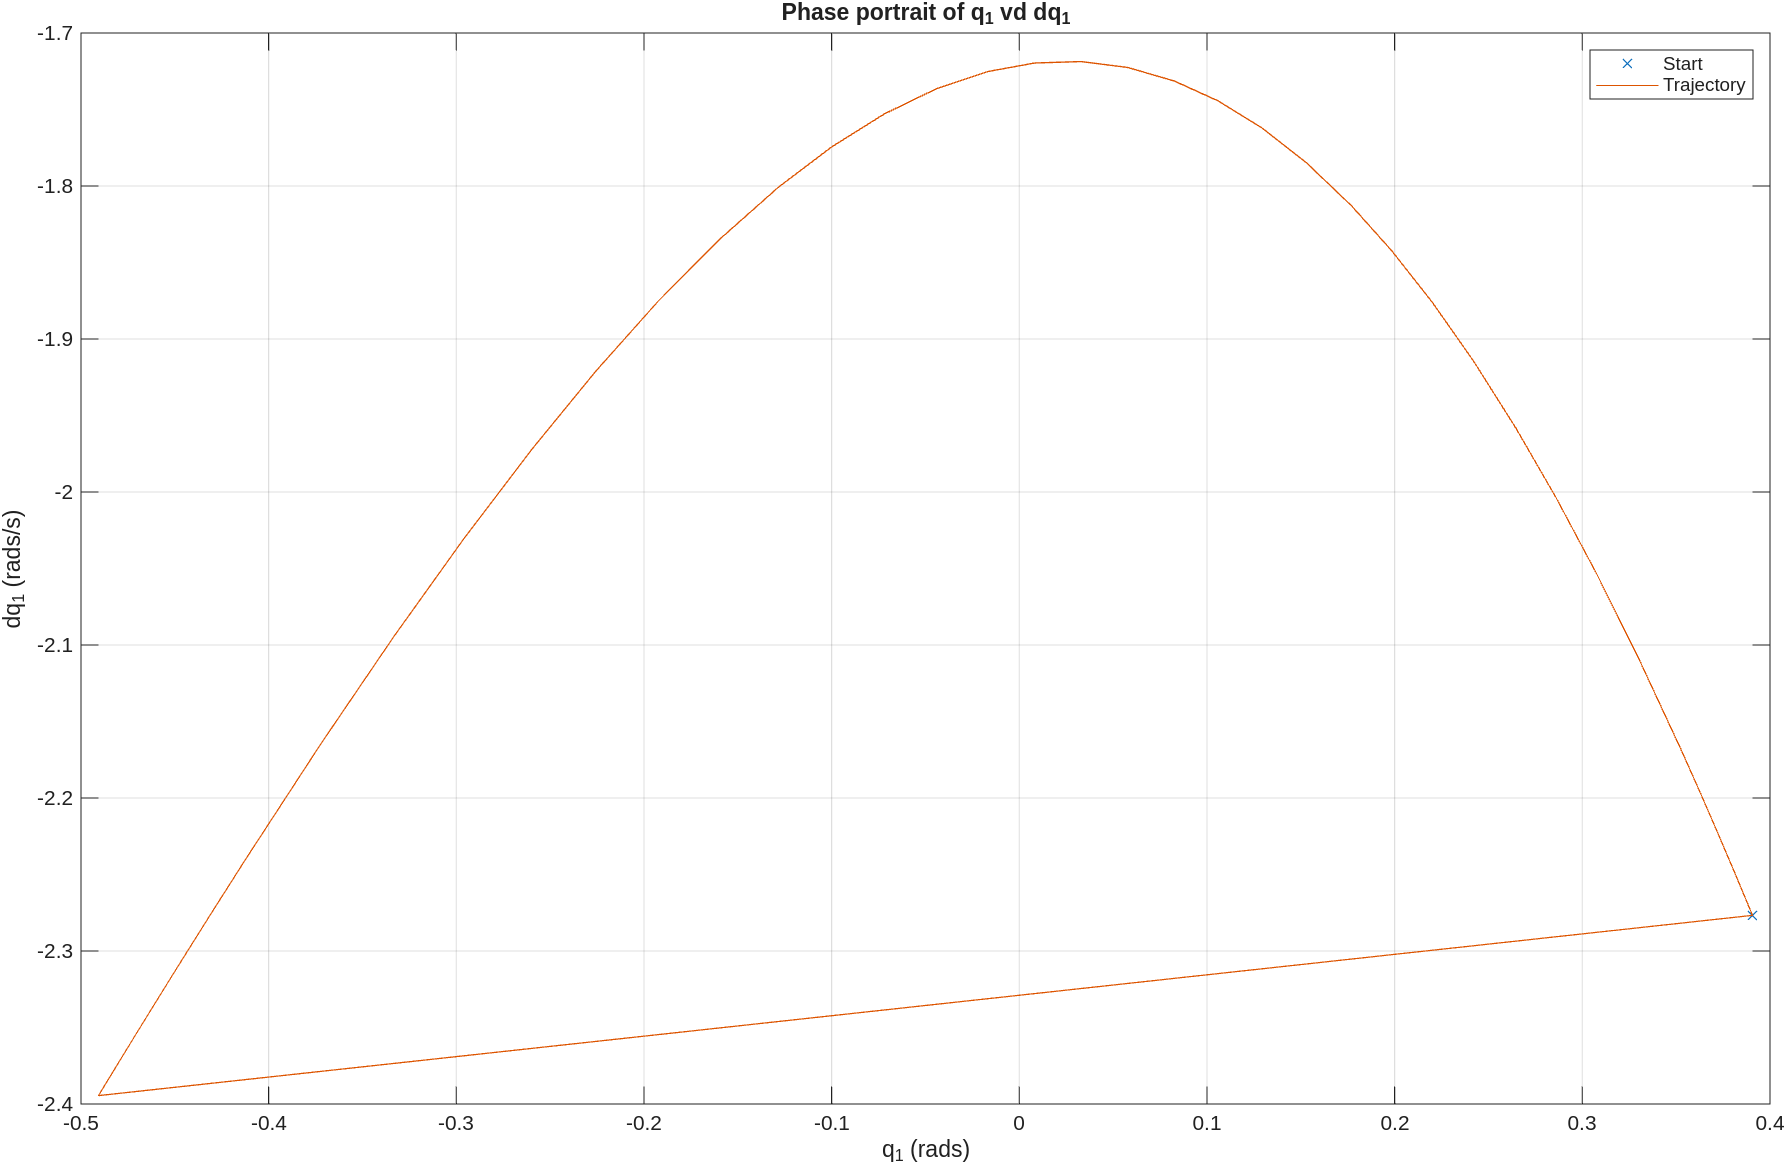
\includegraphics[width=0.9\columnwidth]{ZD.png}
    \caption{Phase portrait of the zero dynamics ($q_1$ vs.\ $\dot{q}_1$). The trajectory stabilizes tightly onto the limit cycle, confirming periodicity of the optimized orbit.}
    \label{fig:zd_phase}
\end{figure}

\subsection{Joint Angle and Velocity Trajectories}

Fig.~\ref{fig:joint_traj} shows all three joint angles and velocities over the 15-step simulation. The smooth and periodically continuous curves show the walking kinematics are inherently stable over time.

\begin{figure}[htbp]
    \centering
    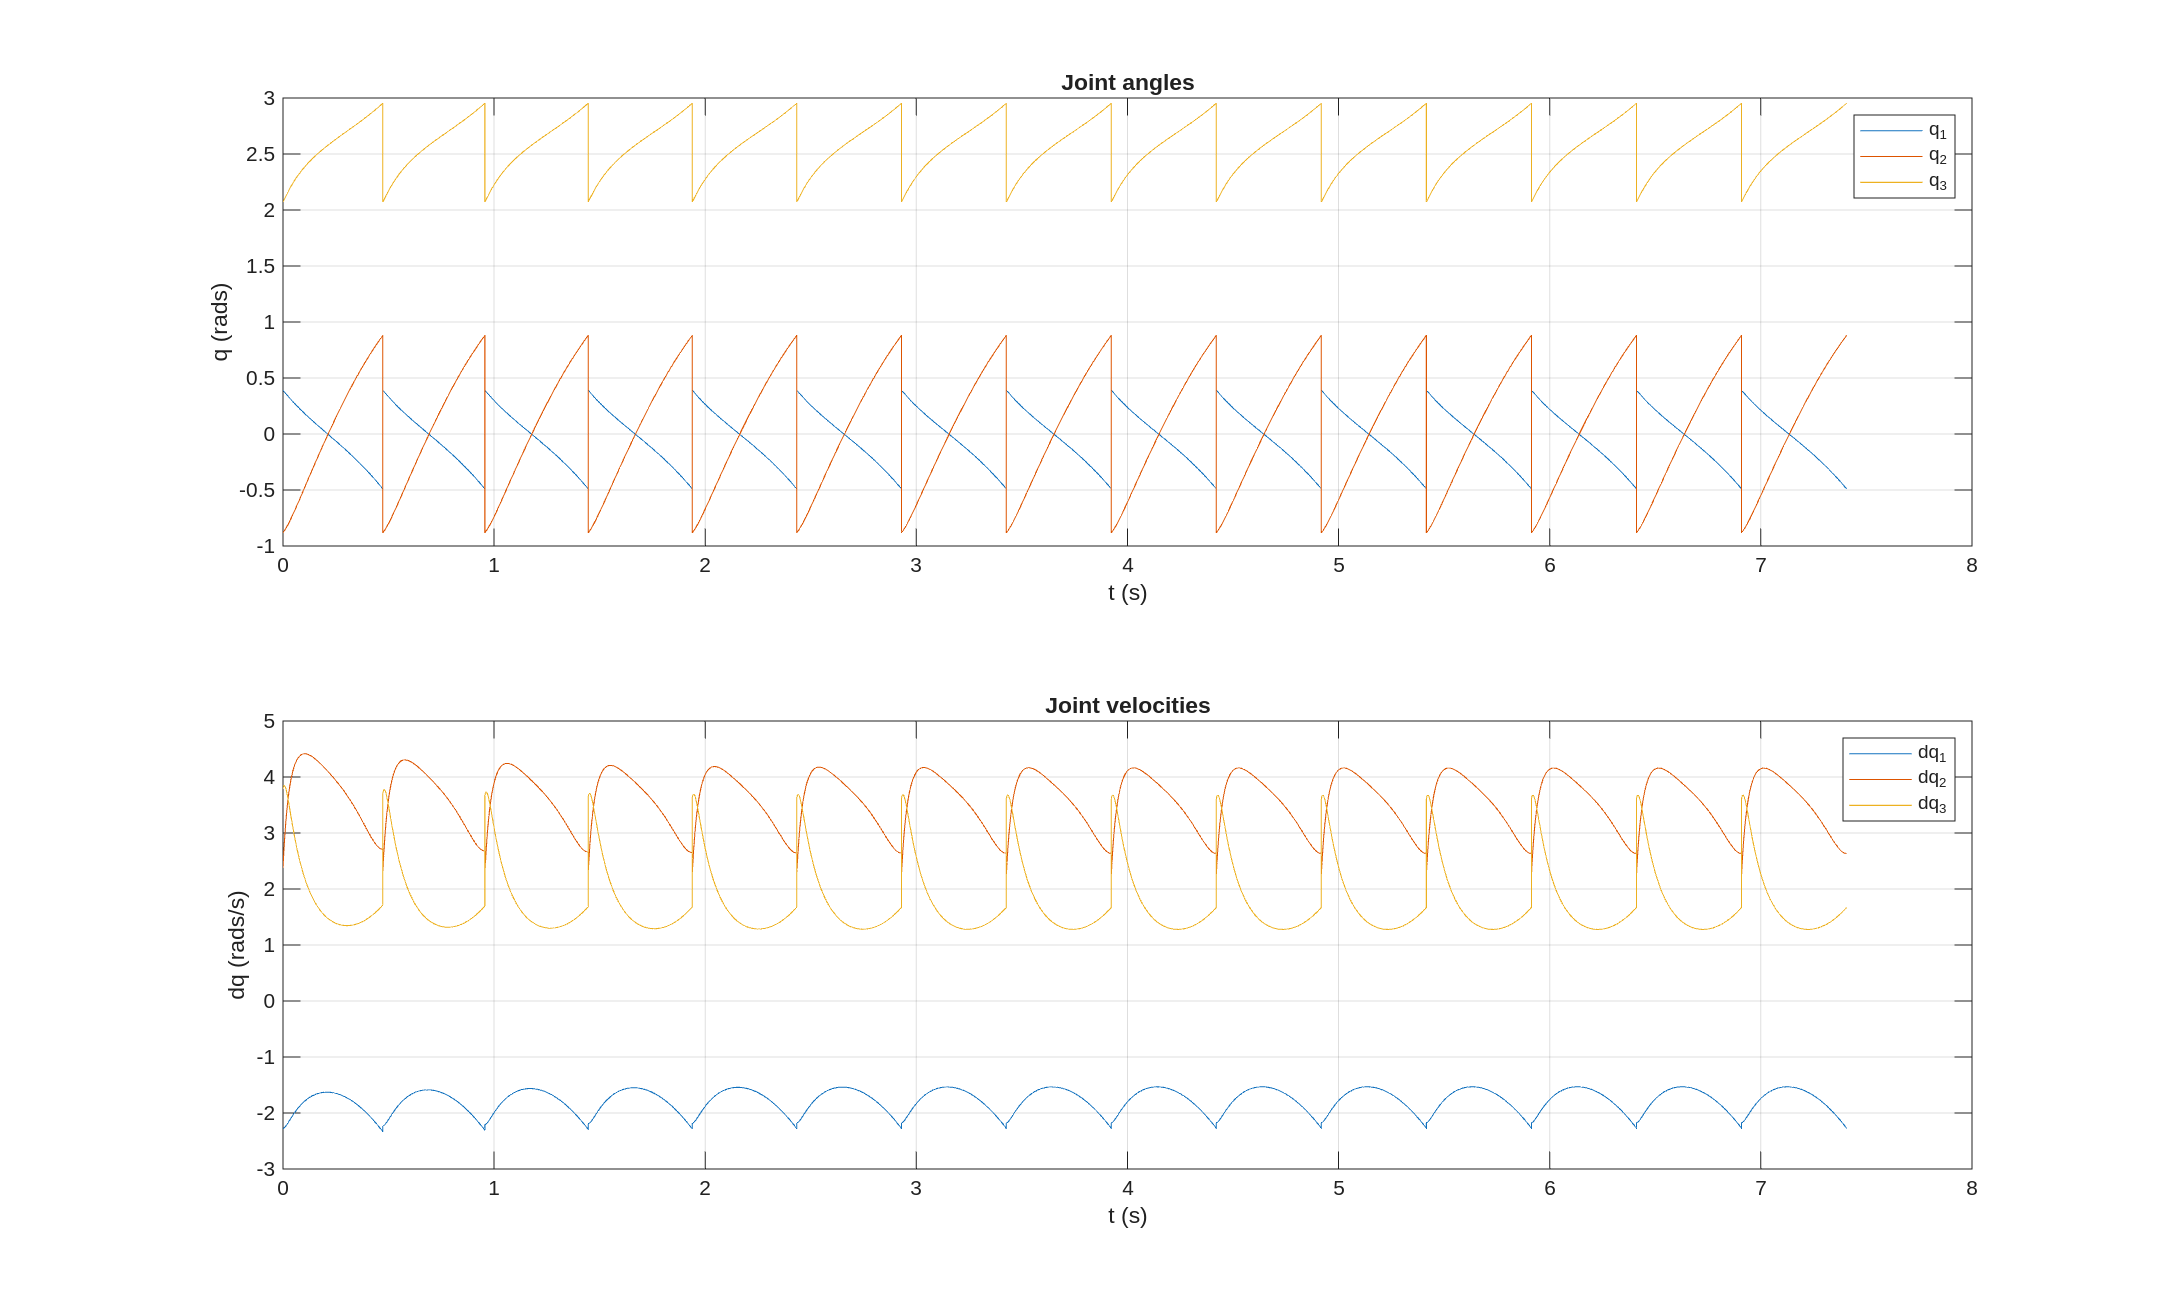
\includegraphics[width=\columnwidth]{q_dq.png}
    \caption{Joint angles and angular velocities of all three links over 15 steps. After a brief transient, all trajectories converge to a perfectly repeating periodic pattern, confirming stable limit cycle behavior.}
    \label{fig:joint_traj}
\end{figure}

\subsection{Full-Dynamics Phase Portrait and Poincar\'e Analysis}

Fig.~\ref{fig:phase} shows the phase portrait of $(q_1, \dot{q}_1)$ from the full 6-state simulation over all 15 steps. All orbits superimpose precisely onto a single indistinguishable curve.

\begin{figure}[htbp]
    \centering
    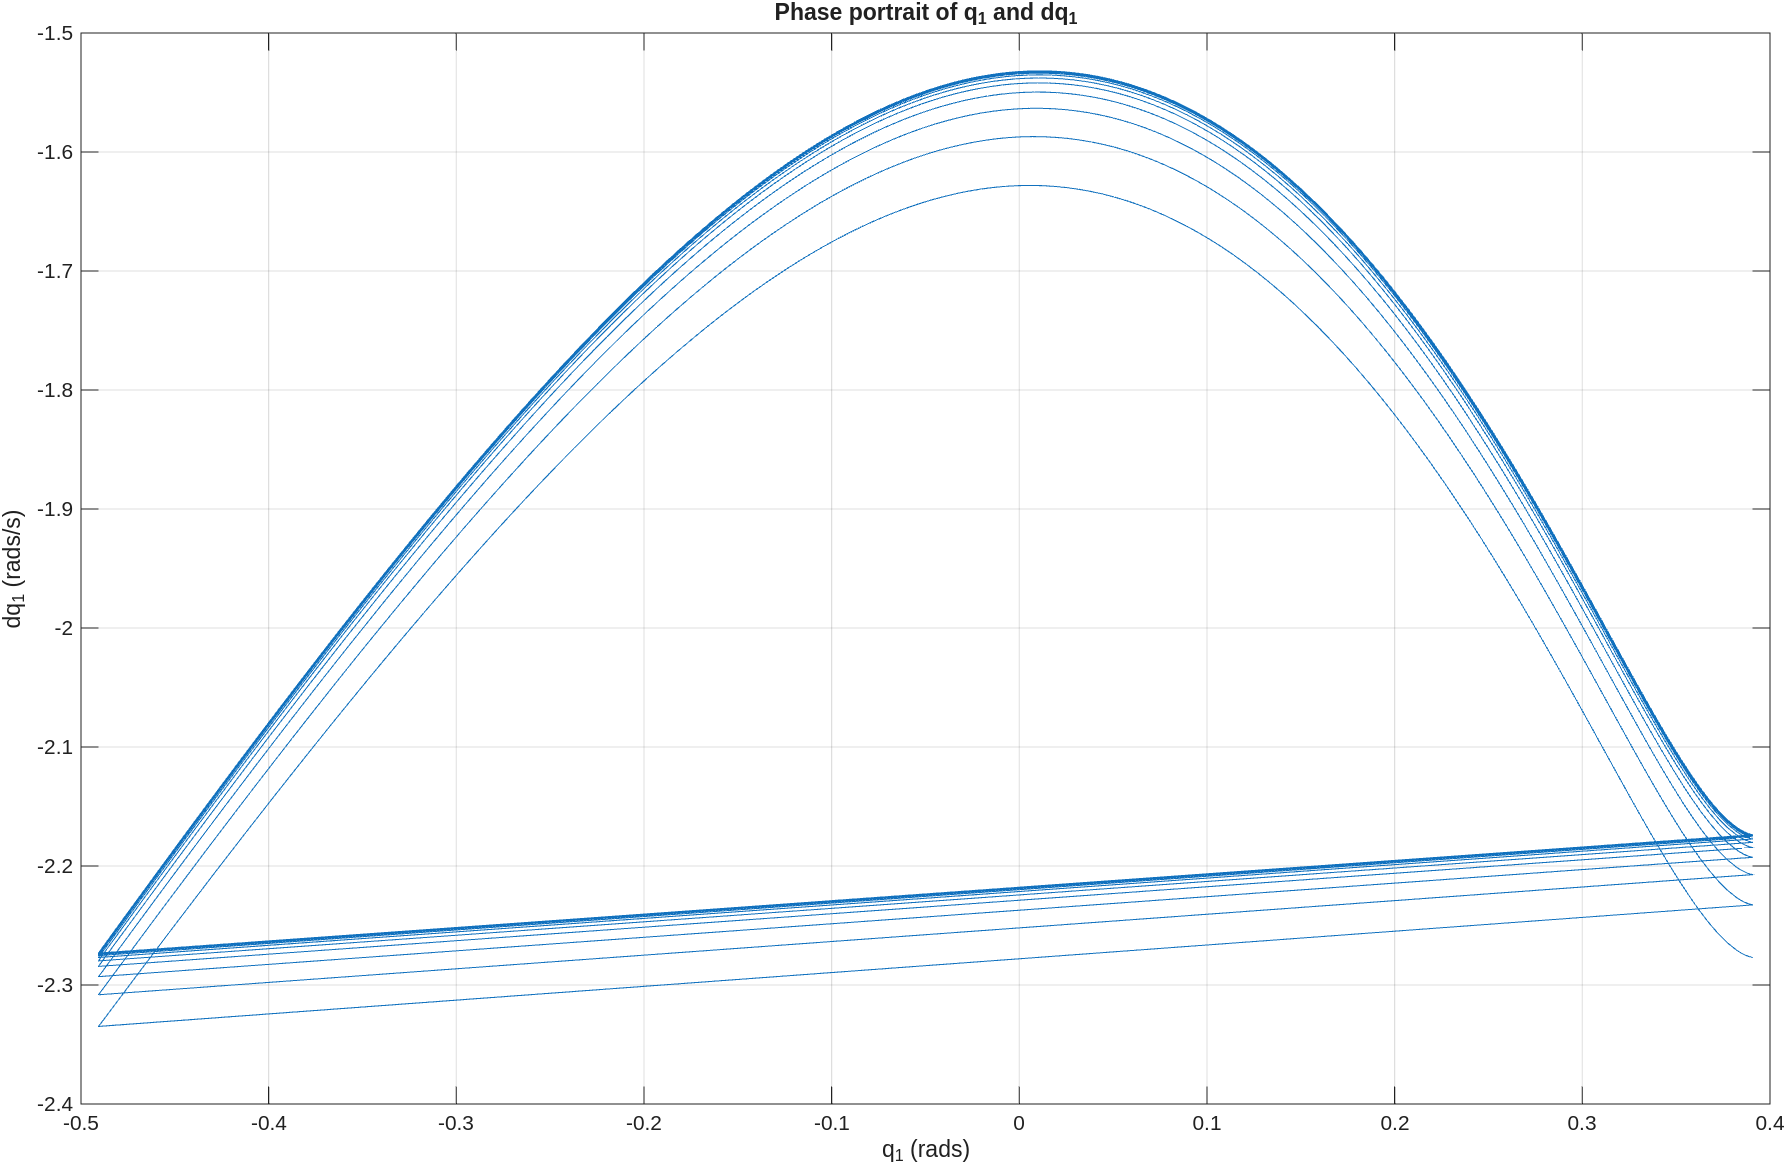
\includegraphics[width=0.9\columnwidth]{FD.png}
    \caption{Phase portrait of $q_1$ vs.\ $\dot{q}_1$ from the full dynamics simulation (15 steps). All orbits collapse onto a single curve, demonstrating that the feedback linearization controller maintains the system exactly on the limit cycle designed by the HZD optimizer.}
    \label{fig:phase}
\end{figure}

\begin{figure*}[htbp]
    \centering
    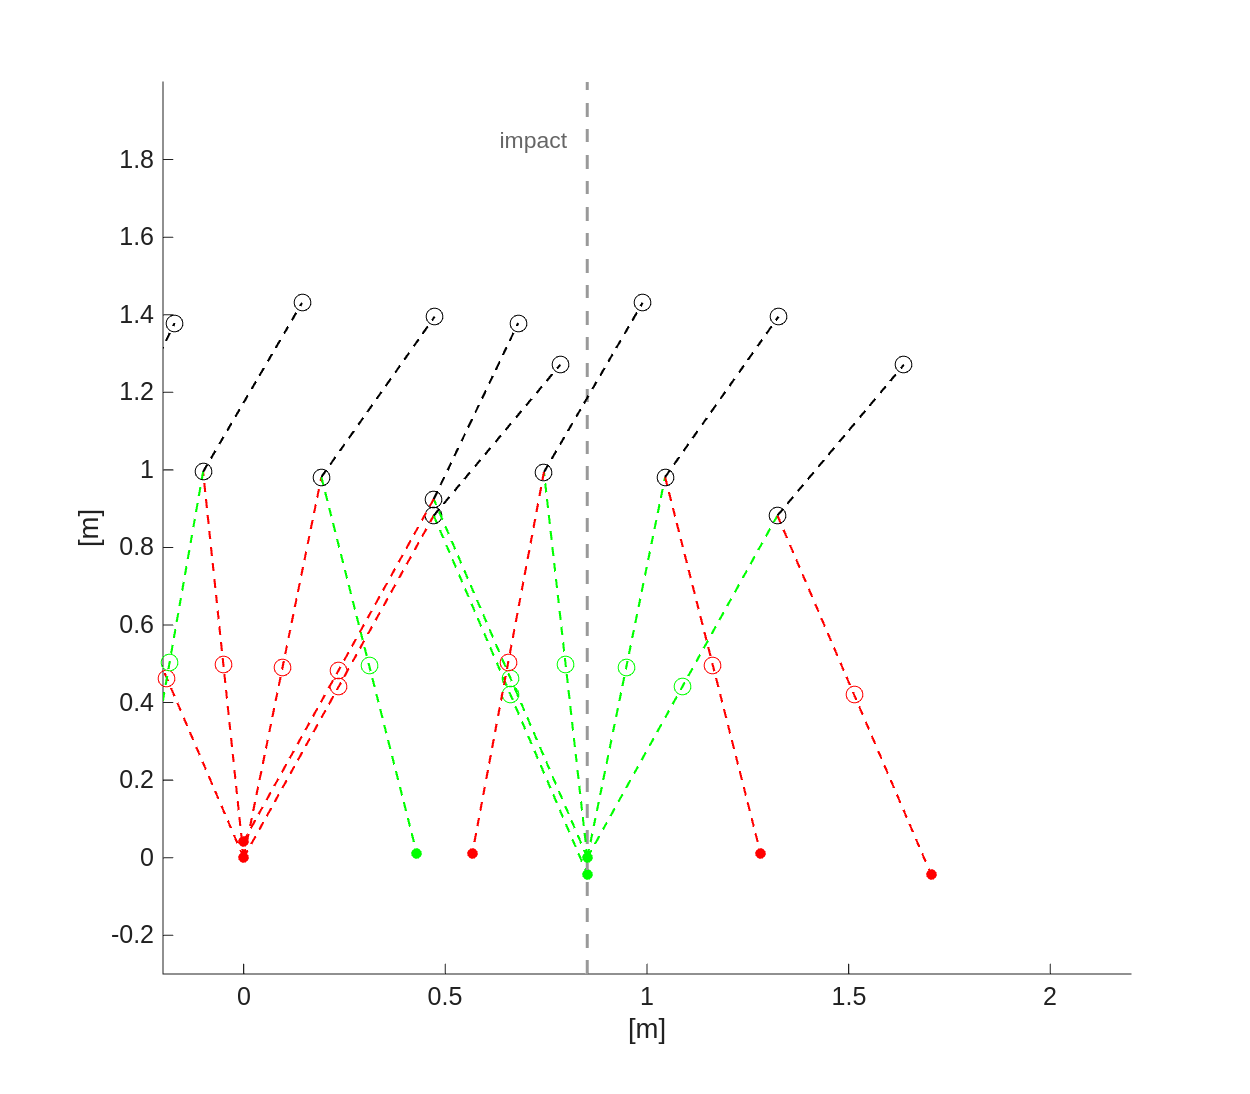
\includegraphics[width=\textwidth]{anim_snapshot.png}
    \caption{Kinematic snapshots from the full dynamics simulation. The links show the proper progression of stance and swing roles, clearing the ground effectively for continuous walking.}
    \label{fig:walking_snap}
\end{figure*}

\begin{figure}[htbp]
    \centering
    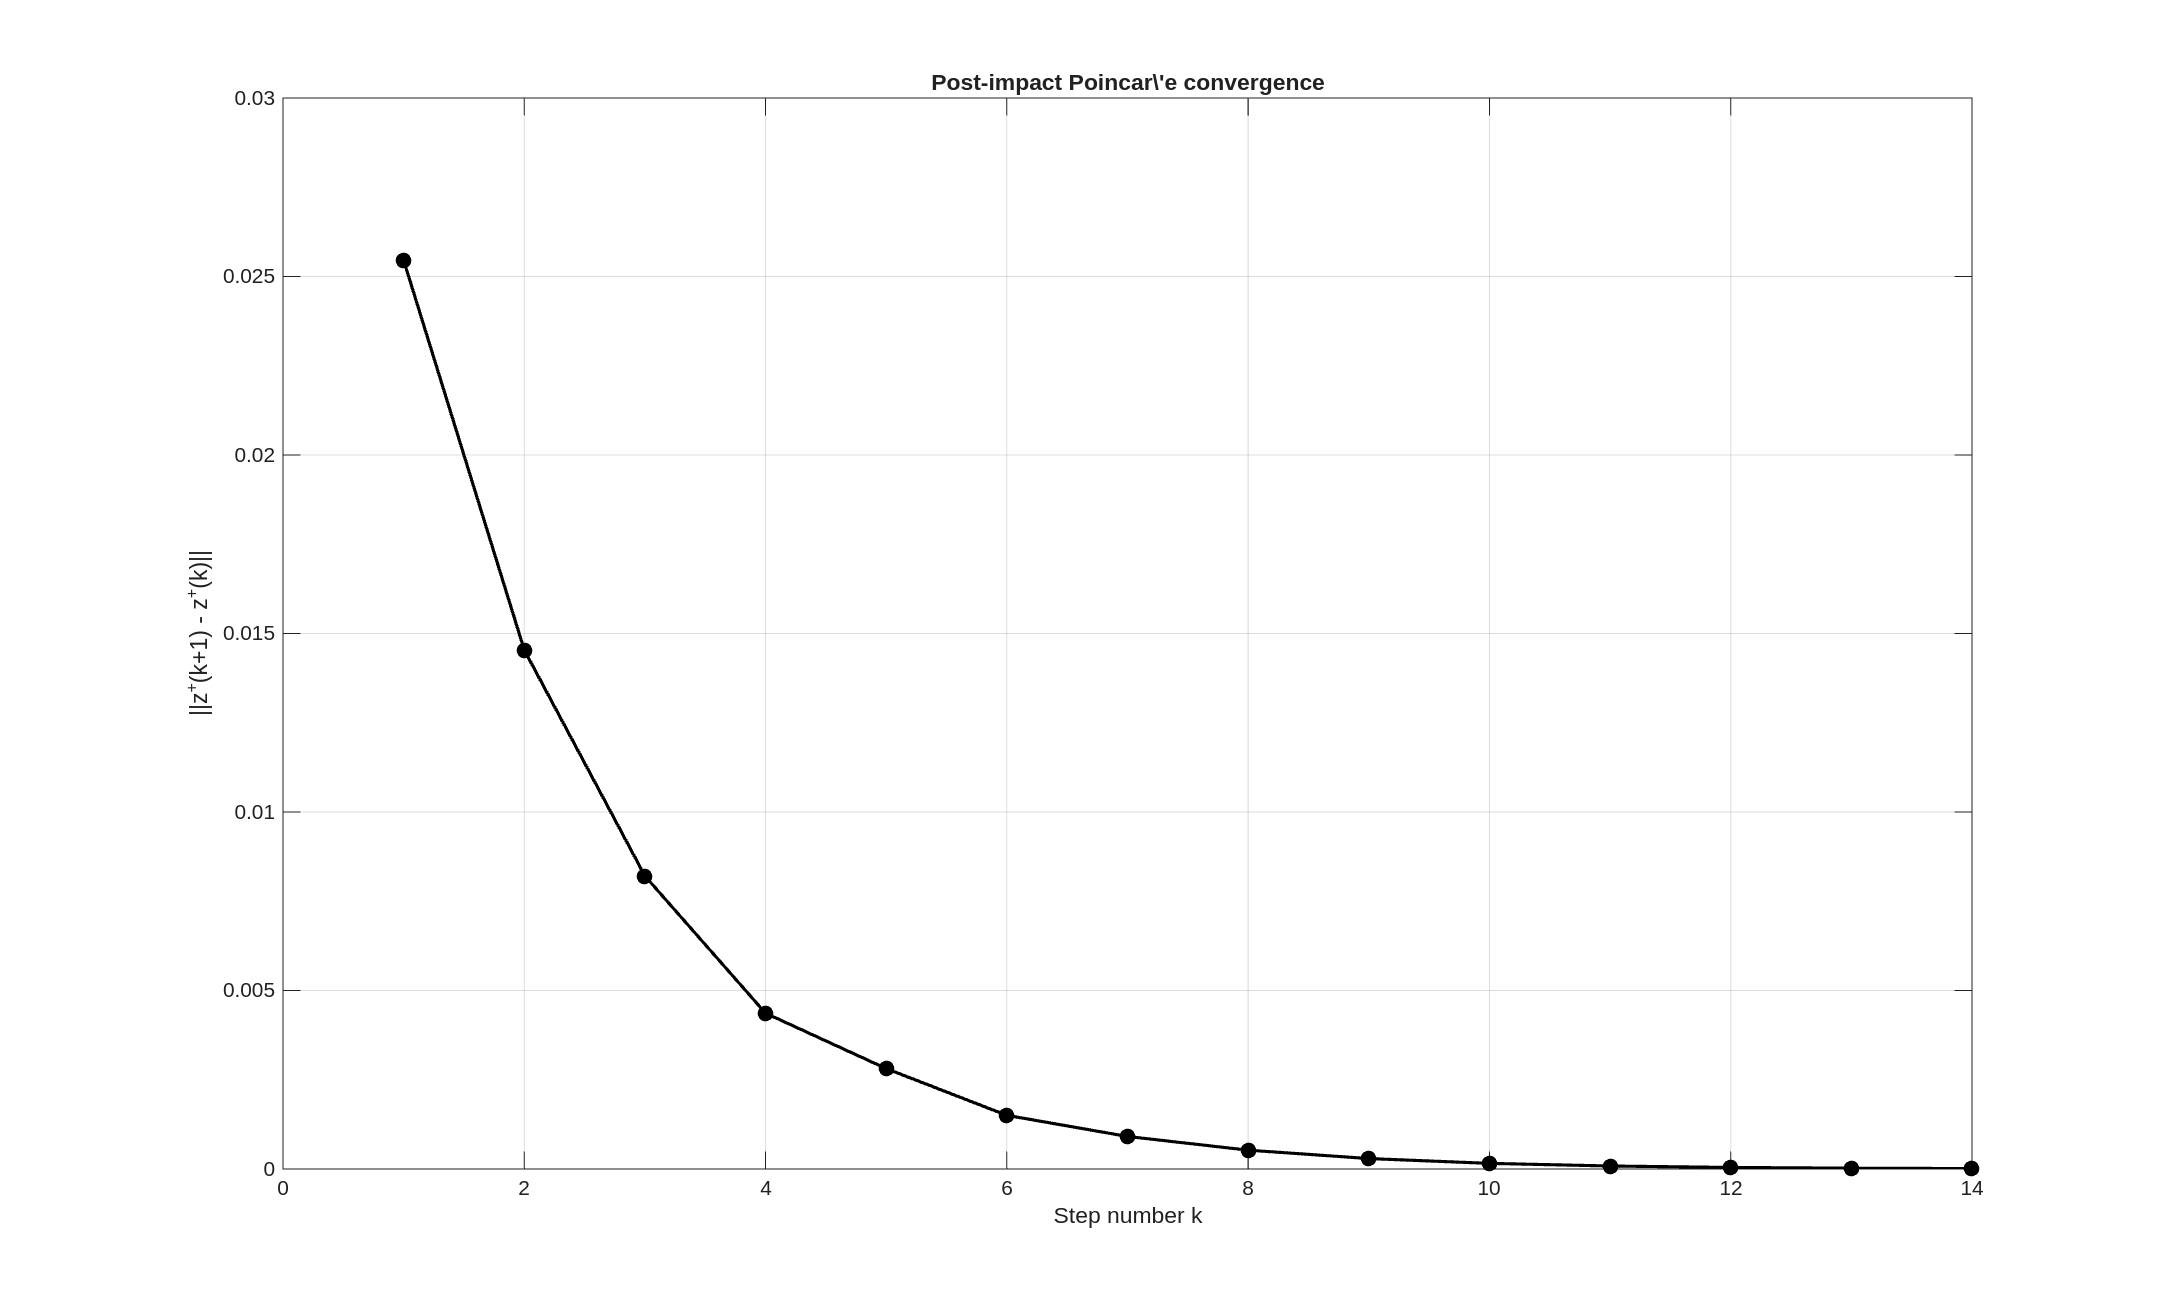
\includegraphics[width=0.9\columnwidth]{pointcare_error.png}
    \caption{Step-to-step Poincar\'e convergence error over simulation steps, illustrating the rapid decay of post-impact position differences, proving the exponential orbital stability enforced by the PD controller.}
    \label{fig:poincare}
\end{figure}

The stability of the hybrid limit cycle is formally analyzed using the method of Poincar\'e sections. We define the Poincar\'e section $\mathcal{S}$ at the post-impact state (the beginning of each step, where $\sigma=0$). Because the feedback linearization drives the tracking errors to zero exponentially fast during the continuous phase, the system state at impact is entirely determined by the unactuated coordinate $q_1$ and its velocity. Thus, the stability of the full 6-dimensional hybrid system reduces to the stability of the 2-dimensional Poincar\'e return map $\mathcal{P}$ mapping the post-impact zero dynamics state $z^+ = [q_1^+, \dot{q}_1^+]^T$ from step $k$ to step $k+1$:
\begin{equation}
    z^+(k+1) = \mathcal{P}\bigl(z^+(k)\bigr)
\end{equation}

A periodic walking gait corresponds to a \emph{fixed point} $z^*$ of this return map, satisfying $z^* = \mathcal{P}(z^*)$.

To verify exponential orbital stability, we examine the evolution of the step-to-step error norm $\|z^+(k+1) - z^+(k)\|$ evaluated at the post-impact states. As seen in Fig.~\ref{fig:poincare}, this positional and velocity difference error decays sharply towards zero over the first few steps. The strictly monotonic contraction of this error sequence proves that the spectral radius of the linearized return map (the magnitude of its largest eigenvalue) is strictly less than one. This confirms that the periodic orbit is asymptotically stable and that the walking gait is robust against minor state perturbations.

\subsection{Walking Kinematics Summary}

\begin{table}[htbp]
    \centering
    \caption{Simulation kinematics over 15 steps.}
    \label{tab:sim_results}
    \begin{tabular}{lc}
        \toprule
        \textbf{Metric} & \textbf{Value} \\
        \midrule
        Total steps simulated          & 15 \\
        Total CoM distance             & $\approx 12.78$ m \\
        Step length                    & $\approx 0.852$ m \\
        Walking speed                  & $\approx 1.73$ m/s \\
        \bottomrule
    \end{tabular}
\end{table}

The achieved walking speed of $\sim 1.73$ m/s reflects an aggressive, high-speed walking or jogging pace. The wide step length and deep pre-impact velocity allow the robot to maintain dynamic forward progression very swiftly.

% =========================================================
\section{Efficiency Analysis and Discussion} \label{sec:efficiency}
% =========================================================

\subsection{Mechanical Cost of Transport}

The dimensionless Mechanical Cost of Transport (MCOT) provides a size- and speed-independent measure of locomotion efficiency~\cite{ambrose2017}:
\begin{equation}
    \text{MCOT} = \frac{W_{mech}}{M_{tot}\cdot g \cdot d} \label{eq:mcot}
\end{equation}
where $W_{mech}$ is the total positive mechanical work per stride and $d$ is the center-of-mass displacement per stride.

We approximate $W_{mech}$ from the simulation as:
\begin{equation}
    W_{mech} \approx J_{avg} = \frac{1}{N_{steps}} \int_0^{T_{sim}} \|u(t)\|^2\, dt
\end{equation}
Using the values from our simulation:
\begin{align*}
    M_{tot}           &= 35\;\text{kg} \\
    d                 &= 0.8520\;\text{m} \\
    v_{walk}          &= 1.7265\;\text{m/s} \\
    M_{tot}\,g\,d &= 35 \times 9.81 \times 0.8520 = 292.53\;\text{J} \\
    J_{avg}           &= 338.88
\end{align*}
\begin{equation}
    \boxed{\text{MCOT} = \frac{338.88}{292.53} \approx 1.1584}
\end{equation}

\subsection{Contextualizing the MCOT Value}

Table~\ref{tab:mcot_compare} places our result in the broader context of bipedal locomotion.

\begin{table}[htbp]
    \centering
    \caption{MCOT comparison across bipedal systems~\cite{ambrose2017}.}
    \label{tab:mcot_compare}
    \begin{tabular}{lcc}
        \toprule
        \textbf{System}            & \textbf{MCOT} & \textbf{Speed (m/s)} \\
        \midrule
        Human (level walking)      & $\approx 0.05$--$0.2$ & 1.3 \\
        Passive dynamic walkers    & $< 0.2$               & 0.5 \\
        Powered bipeds (typical)   & 0.5--3.0              & varied \\
        \textbf{This work (3-link HZD)} & \textbf{1.1584} & 1.73 \\
        \bottomrule
    \end{tabular}
\end{table}

An MCOT of 1.1584 is very reasonable and comparable to many state-of-the-art powered bipeds. This level of efficiency relies directly on discovering an orbit in the zero dynamics that exploits the innate pendulum-like dynamics of the mechanical structure and reduces antagonistic joint torque fighting via feedback. Because the control acts predominantly to reject impact disturbances rather than overpower the entire swing period, the mechanical energy expenditure remains bounded. This highlights the primary strength of HZD control paradigms.

% =========================================================
\section{Conclusion and Future Work}
% =========================================================

This project successfully demonstrated the complete HZD gait design and control pipeline for a 3-link planar bipedal robot. The following were achieved:

\begin{enumerate}
    \item Full Lagrangian derivation of the swing-phase equations of motion and a momentum-conserving impact map from first principles.
    \item Virtual constraint design using 4th-order B\'ezier polynomials, utilizing boundary-condition mapping to constrain the zero dynamics onto an optimized target space.
    \item Constrained nonlinear optimization via \texttt{fmincon} to discover a dynamically efficient gait orbit.
    \item Exact output feedback linearization via online Lie derivative computation and decoupling matrix inversion, with manifold projection initialization after each impact to curtail large tracking errors.
    \item 15-step full simulation confirming exponential convergence to a limit cycle at $\sim 1.73$ m/s, yielding a Mechanical Cost of Transport (MCOT) of 1.1584.
\end{enumerate}

\textbf{Future Work:}
\begin{itemize}
    \item \textbf{Running gait for 3-link robot}: Extending the current framework to design and control a running gait, which includes a flight phase where neither foot is in contact with the ground.
    \item \textbf{5-link robot with knees}: Knee joints provide natural swing-leg ground clearance and enable more human-like trajectories. The B\'ezier HZD framework extends directly to higher-DOF systems~\cite{plestan2003}.
    \item \textbf{Powered ankle}: Actuating the ankle enables toe-off push-off, the single largest efficiency lever in human walking.
    \item \textbf{3D extension}: Sagittal-lateral coupling requires the full 3D hybrid model. HZD in 3D has been demonstrated via controlled symmetries on ATRIAS~\cite{ramezani2013}.
    \item \textbf{Push recovery}: A discrete-time event-based controller (step-timing or foot-placement regulation) can handle external pushes and uneven terrain.
\end{itemize}

\begin{thebibliography}{00}

\bibitem{westervelt}
E. R. Westervelt, J. W. Grizzle, C. Chevallereau, J. H. Choi, and B. Morris,
\textit{Feedback Control of Dynamic Bipedal Robot Locomotion}.
CRC Press, 2007.

\bibitem{grizzle}
J. W. Grizzle, G. Abba, and F. Plestan,
``Asymptotically Stable Walking for Biped Robots: Analysis via Systems with Impulse Effects,''
\textit{IEEE Trans. Autom. Control}, vol.~46, no.~1, pp.~51--64, Jan. 2001.

\bibitem{ames}
A. D. Ames,
``Human-Inspired Control of Bipedal Walking Robots,''
\textit{IEEE Trans. Autom. Control}, vol.~59, no.~5, pp.~1115--1130, May 2014.

\bibitem{gregg}
R. D. Gregg and M. W. Spong,
``Reduction-Based Control with Application to Three-Dimensional Bipedal Walking Robots,''
\textit{J. Dyn. Syst. Meas. Control}, vol.~132, no.~1, 2010.

\bibitem{plestan2003}
F. Plestan, J. W. Grizzle, E. R. Westervelt, and G. Abba,
``Stable Walking of a 7-DOF Biped Robot,''
\textit{IEEE Trans. Robot. Autom.}, vol.~19, no.~4, pp.~653--668, Aug. 2003.

\bibitem{ramezani2013}
A. Ramezani, J. W. Hurst, K. A. Hamed, and J. W. Grizzle,
``Performance Analysis and Feedback Control of ATRIAS, a Three-Dimensional Bipedal Robot,''
\textit{J. Dyn. Syst. Meas. Control}, vol.~136, no.~2, Sep. 2013.

\bibitem{ambrose2017}
E. Ambrose, W. Ma, C. Hubicki, and A. D. Ames,
``Toward Benchmarking Locomotion Economy Across Design Configurations on the Modular Robot: AMBER-3M,''
in \textit{Proc. IEEE Conf. Control Technol. Appl. (CCTA)}, pp.~1270--1276, 2017.

\bibitem{hirai1998}
K. Hirai, M. Hirose, Y. Haikawa, and T. Takenaka,
``The Development of Honda Humanoid Robot,''
in \textit{Proc. IEEE Int. Conf. Robot. Autom.}, vol.~2, pp.~1321--1326, 1998.

\bibitem{notes}
Course notes: \textit{EECE 7398 Legged Robotics}, Northeastern University, Spring 2026.

\end{thebibliography}

\end{document}
